\section{Ilham Muhammad Ariq D4TI2C 1174087}
\subsection{Keterampilan Pemrograman}
\begin{enumerate}
    \item Buatlah  fungsi  (file  terpisah/library  dengan  nama  \verb|NPM_csv.py|)  untuk  membuka file csv dengan lib csv mode list.
    
    \lstinputlisting[firstline=8, lastline=14]{src/4/1174087/Praktek/1174087_csv.py}

    \item Buatlah  fungsi  (file  terpisah/library  dengan  nama  \verb|NPM_csv.py|)  untuk  membuka file csv dengan lib csv mode dictionary.
   	
   	\lstinputlisting[firstline=16, lastline=20]{src/4/1174087/Praktek/1174087_csv.py}

	\item Buatlah fungsi (file terpisah/library dengan nama \verb|NPM_pandas.py|) untuk membuka file csv dengan lib pandas mode list.
	
	\lstinputlisting[firstline=7, lastline=11]{src/4/1174087/Praktek/1174087_pandas.py}
		
	\item Buatlah fungsi (file terpisah/library dengan nama \verb|NPM_pandas.py| untuk membuka file csv dengan lib pandas mode dictionary.

	\lstinputlisting[firstline=13, lastline=16]{src/4/1174087/Praktek/1174087_pandas.py}

	\item Buat fungsi baru di \verb|NPM_pandas.py| untuk mengubah format tanggal menjadi standar dataframe.

	\lstinputlisting[firstline=25, lastline=27]{src/4/1174087/Praktek/1174087_pandas.py}

	\item Buat fungsi baru di \verb|NPM_pandas.py| untuk mengubah index kolom.
	
	\lstinputlisting[firstline=29, lastline=32]{src/4/1174087/Praktek/1174087_pandas.py}
	
	\item Buat fungsi baru di \verb|NPM_pandas.py| untuk mengubah atribut atau nama kolom.
	
	\lstinputlisting[firstline=34, lastline=37]{src/4/1174087/Praktek/1174087_pandas.py}
	
	\item Buat program main.py yang menggunakan library \verb|NPM_csv.py| yang membuat dan membaca file csv.
	
	\lstinputlisting[firstline=8, lastline=15]{src/4/1174087/Praktek/main.py}
	
	\item Buat program main2.py yang menggunakan library \verb|NPM_pandas.py| yang membuat dan membaca file csv.

	\lstinputlisting[firstline=8, lastline=12]{src/4/1174087/Praktek/main2.py}
\end{enumerate} 

\subsection{Keterampilan Penanganan Error}

\begin{enumerate}
	\item Tuliskan peringatan error yang didapat dari mengerjakan praktek ketiga ini,
dan jelaskan cara penanganan error tersebut. dan Buatlah satu fungsi yang
menggunakan gunakan try except untuk menanggulangi error tersebut.

	\lstinputlisting[firstline=7, lastline=16]{src/4/1174087/Praktek/error.py}
	
	\par NameError adalah exception yang terjadi saat kode melakukan eksekusi terhadap local name atau global name yang tidak terdefinisi. Misalnya saat menjumlahkan variable yang tidak didefinisikan, memanggil function yang tidak ada, dan lain-lain.
	
\end{enumerate}

\textbf{Screenshoot Kode Program Python}

\begin{figure}[H]
 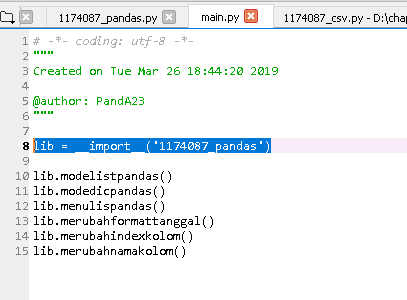
\includegraphics[width=5cm]{figures/4/1174087/Praktek/main.png}
 \centering
\end{figure}

\begin{figure}[H]
 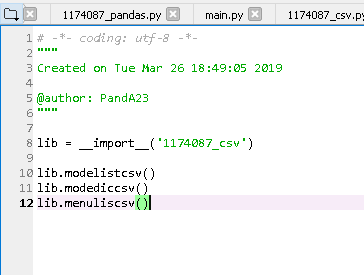
\includegraphics[width=5cm]{figures/4/1174087/Praktek/main2.png}
 \centering
\end{figure}

\begin{figure}[H]
 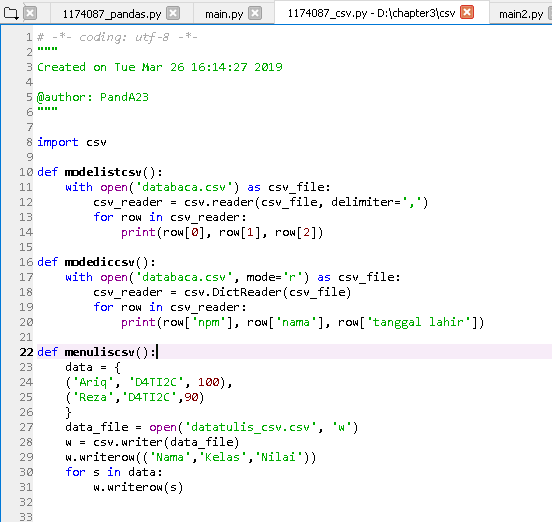
\includegraphics[width=5cm]{figures/4/1174087/Praktek/1174087_csv.png}
 \centering
\end{figure}

\begin{figure}[H]
 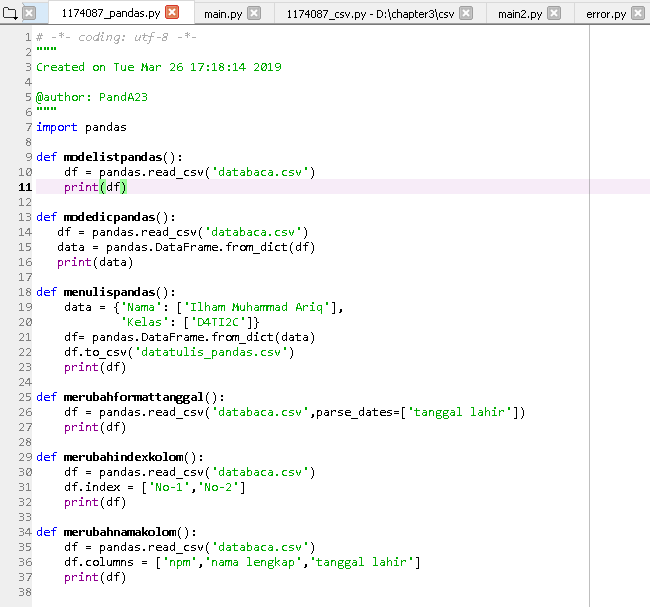
\includegraphics[width=5cm]{figures/4/1174087/Praktek/1174087_pandas.png}
 \centering
\end{figure}

\begin{figure}[H]
 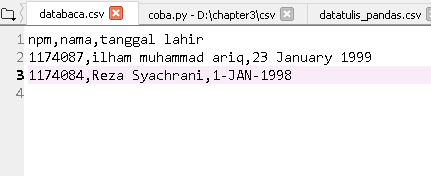
\includegraphics[width=5cm]{figures/4/1174087/Praktek/databaca.png}
 \centering
\end{figure}

\begin{figure}[H]
 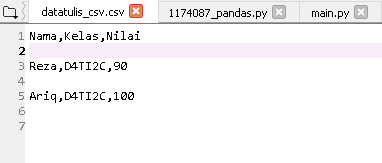
\includegraphics[width=5cm]{figures/4/1174087/Praktek/datatulis_csv.png}
 \centering
\end{figure}

\begin{figure}[H]
 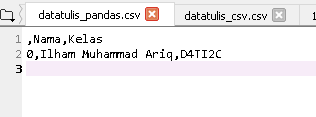
\includegraphics[width=5cm]{figures/4/1174087/Praktek/datatulis_pandas.png}
 \centering
\end{figure}

\begin{figure}[H]
 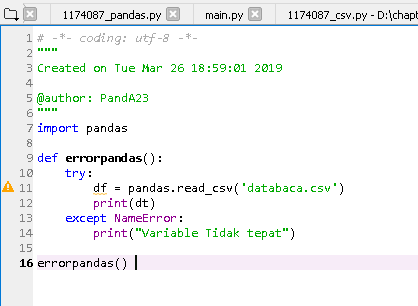
\includegraphics[width=5cm]{figures/4/1174087/Praktek/error.png}
 \centering
\end{figure}

%%%%%%%%%%%%%%%%%%%%%%%%%%%%%%%%%%%%%%%%%%%%%%%%%%%%%%%%%%%%%%%%%%%%%%%%%%%%%%%%%%%%%%%%%%%%%%%%%%%%%%%%%%%%%%%%%%%%%%
\section{Dini Permata Putri | 1174053}
\subsection{Keterampilan Pemrograman}
\begin{enumerate}
\item Buatlah  fungsi  (file  terpisah/library  dengan  nama  NPMcsv.py)  untuk  membuka file csv dengan lib csv mode list.


	\lstinputlisting[firstline=10, lastline=15]{src/4/1174053/Praktek/1174053csv.py}

	\item Buatlah  fungsi  (file  terpisah/library  dengan  nama  NPMcsv.py)  untuk  membuka file csv dengan lib csv mode dictionary.

	\lstinputlisting[firstline=17, lastline=22]{src/4/1174053/Praktek/1174053csv.py}

	\item Buatlah fungsi (file terpisah/library dengan nama NPMpandas.py) untuk membuka file csv dengan lib pandas mode list.

	\lstinputlisting[firstline=10, lastline=13]{src/4/1174053/Praktek/1174053pandas.py}

	\item Buatlah fungsi (file terpisah/library dengan nama NPMpandas.py) untuk membuka file csv dengan lib pandas mode dictionary.

	\lstinputlisting[firstline=10, lastline=13]{src/4/1174053/Praktek/1174053pandas.py}

	\item  Buat fungsi baru di NPMpandas.py untuk mengubah format tanggal menjadi standar dataframe.

	\lstinputlisting[firstline=15, lastline=19]{src/4/1174053/Praktek/1174053pandas.py}

	\item Buat fungsi baru di NPMpandas.py untuk mengubah index kolom.

	\lstinputlisting[firstline=21, lastline=24]{src/4/1174053/Praktek/1174053pandas.py}

	\item Buat fungsi baru di NPMpandas.py untuk mengubah atribut atau nama kolom.

	\lstinputlisting[firstline=26, lastline=30]{src/4/1174053/Praktek/1174053pandas.py}

	\item Buat program main.py yang menggunakan library NPMcsv.py yang membuat dan membaca file csv.

	\lstinputlisting[firstline=8, lastline=13]{src/4/1174053/Praktek/main.py}

	\item Buat program main2.py yang menggunakan library NPMpandas.py yang membuat dan membaca file csv.

	\lstinputlisting[firstline=8, lastline=13]{src/4/1174053/Praktek/main2.py}
\end{enumerate}

\subsection{Penanganan Error}
Peringatan error di praktek keempat ini, yaitu:
	\begin{itemize}
		\item Syntax Errors
		Syntax Error, adalah kesalahan yang disebabkan oleh kesalahan tata cara penulisan tanda baca, kesalahan pemakaian operator dan nilai. Kesalahan jenis ini akan dengan mudah dideteksi oleh kompiler maupun interpreter.

		\item Name Error
		NameError adalah exception yang terjadi saat kode melakukan eksekusi terhadap local name atau global name yang tidak terdefinisi. Misalnya saat menjumlahkan variable yang tidak didefinisikan, memanggil function yang tidak ada, dan lain-lain.

		\item Type Error
		TypeError adalah exception yang akan terjadi apabila pada saat dilakukannya eksekusi terhadap suatu operasi atau fungsi dengan type object yang tidak sesuai. Solusi dari error ini adalah mengkoversi varibelnya sesuai dengan tipe data yang akan digunakan.
	

	\item Fungsi yang menggunakan try except
	\lstinputlisting[firstline=55, lastline=67]{src/4/1174053/Praktek/1174053.py}
\end{itemize}


%%%%%%%%%%%%%%%%%%%%%%%%%%%%%%%%%%%%%%%%%%%%%%%%%%%%%%%%%%%%%%%%%%%%%%%%%%%%%%%%%%%%%%%%%%%%%%%%%%
\section{Bakti Qilan Mufid | 1174083}
\subsection{Soal 1}
Jawaban soal ke-1

\lstinputlisting[caption =  Fungsi untuk membuka file CSV dengan lib CSV mode list.,firstline=11, lastline=16]{src/4/1174083/Praktek/1174083_csv.py}

\subsection{Soal 2}
Jawaban soal ke-2

\lstinputlisting[caption =  Fungsi untuk membuka file CSV dengan lib CSV mode dictionary., firstline=18, lastline=23]{src/4/1174083/Praktek/1174083_csv.py}

\subsection{Soal 3}
Jawaban soal ke-3

\lstinputlisting[caption =  Fungsi untuk membuka file CSV dengan lib Pandas mode list., firstline=11, lastline=14]{src/4/1174083/Praktek/1174083_pandas.py}

\subsection{Soal 4}
Jawaban soal ke-4

\lstinputlisting[caption =  Fungsi untuk membuka file CSV dengan lib Pandas mode dictionary., firstline=16, lastline=20]{src/4/1174083/Praktek/1174083_pandas.py}

\subsection{Soal 5}
Jawaban soal ke-5

\lstinputlisting[caption =  Fungsi untuk mengubah format tanggal menjadi standar dataframe., firstline=22, lastline=25]{src/4/1174083/Praktek/1174083_pandas.py}

\subsection{Soal 6}
Jawaban soal ke-6

\lstinputlisting[caption =  Fungsi untuk mengubah index kolom., firstline=21, lastline=24]{src/4/1174083/Praktek/1174083_pandas.py}

\subsection{Soal 7}
Jawaban soal ke-7

\lstinputlisting[caption =  Fungsi untuk mengubah atribut atau nama kolom., firstline=33, lastline=37]{src/4/1174083/Praktek/1174083_pandas.py}

\subsection{Soal 8}
Jawaban soal ke-8

\lstinputlisting[caption =  Membuat dan membaca file CSV menggunakan library 1174083pandas., firstline=8, lastline=13]{src/4/1174083/Praktek/main.py}

\subsection{Soal 9}
Jawaban soal ke-9

\lstinputlisting[caption = Membuat dan membaca file CSV menggunakan library 1174083pandas., firstline=8, lastline=13]{src/4/1174083/Praktek/main2.py}

\subsection{Bukti Screenshoot}

\begin{figure}[H]
	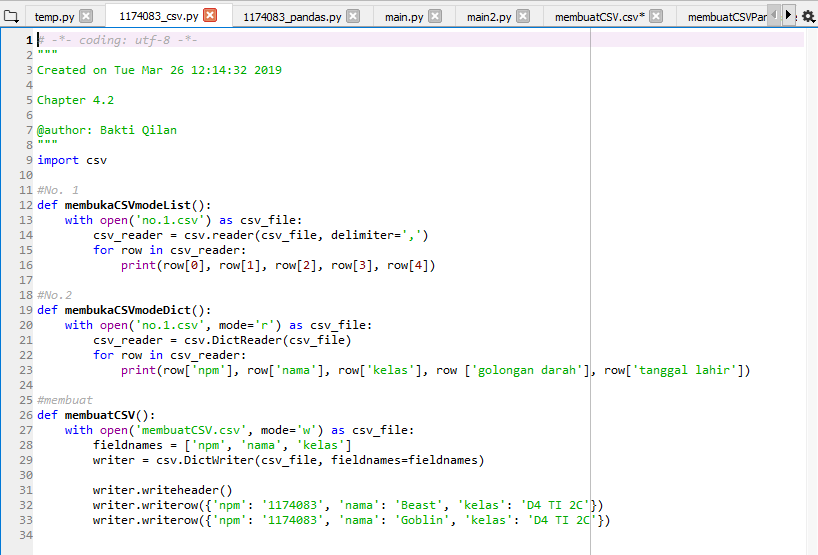
\includegraphics[width=10cm]{figures/4/1174083/Praktek/kode_praktek_1.png}
	\centering
\end{figure}

\begin{figure}[H]
	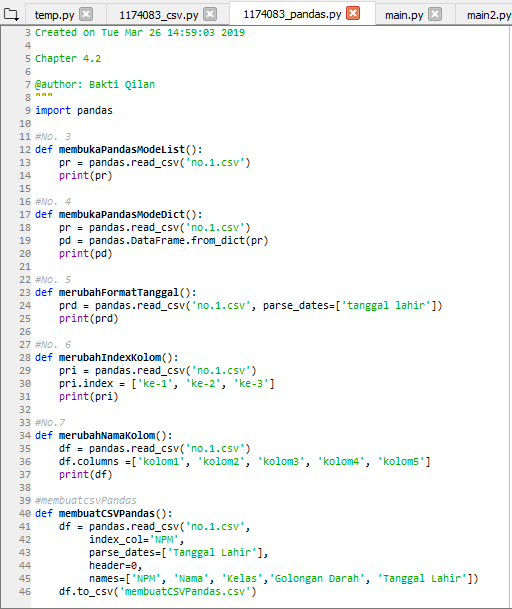
\includegraphics[width=10cm]{figures/4/1174083/Praktek/kode_praktek_2.png}
	\centering
\end{figure}

\begin{figure}[H]
	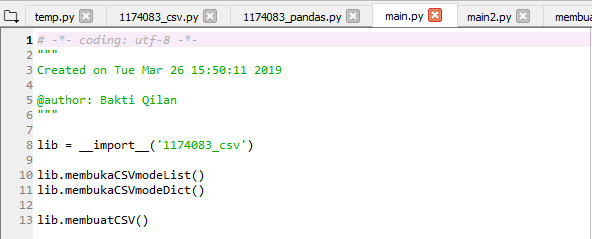
\includegraphics[width=10cm]{figures/4/1174083/Praktek/kode_praktek_3.png}
	\centering
\end{figure}

\begin{figure}[H]
	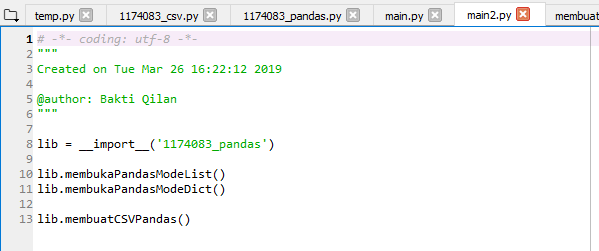
\includegraphics[width=10cm]{figures/4/1174083/Praktek/kode_praktek_4.png}
	\centering
\end{figure}

\begin{figure}[H]
	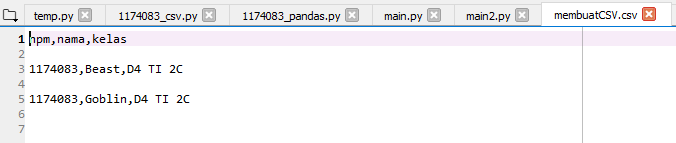
\includegraphics[width=10cm]{figures/4/1174083/Praktek/kode_praktek_5.png}
	\centering
\end{figure}

\begin{figure}[H]
	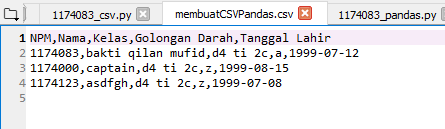
\includegraphics[width=10cm]{figures/4/1174083/Praktek/kode_praktek_6.png}
	\centering
\end{figure}

\begin{figure}[H]
	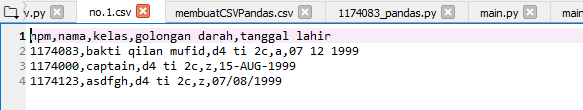
\includegraphics[width=10cm]{figures/4/1174083/Praktek/kode_praktek_7.png}
	\centering
\end{figure}

%%%%%%%%%%%%%%%%%%%%%%%%%%%%%%%%%%%%%%%%%%%%%%%%%%%%%%%%%%%%%%%%%%%%%%%%%%%%%%

\section{Muhammad Reza Syachrani / 1174084}
\subsection{Soal 1}
jawaban : \lstinputlisting[caption=Jawaban no.1, firstline=10, lastline=14, ]{src/4/1174084/Praktek/chapter4/1174084_csv.py}

\subsection{Soal 2}
jawaban : \lstinputlisting[caption=Jawaban no.2, firstline=18, lastline=22, ]{src/4/1174084/Praktek/chapter4/1174084_csv.py}

\subsection{Soal 3}
jawaban : \lstinputlisting[caption=Jawaban no.3, firstline=11, lastline=13, ]{src/4/1174084/Praktek/chapter4/1174084_pandas.py}

\subsection{Soal 4}
jawaban : \lstinputlisting[caption=Jawaban no.4, firstline=17, lastline=20, ]{src/4/1174084/Praktek/chapter4/1174084_pandas.py}

\subsection{Soal 5}
jawaban : \lstinputlisting[caption=Jawaban no.5, firstline=24, lastline=26, ]{src/4/1174084/Praktek/chapter4/1174084_pandas.py}

\subsection{Soal 6}
jawaban : \lstinputlisting[caption=Jawaban no.6, firstline=30, lastline=33, ]{src/4/1174084/Praktek/chapter4/1174084_pandas.py}

\subsection{Soal 7}
jawaban : \lstinputlisting[caption=Jawaban no.7, firstline=37, lastline=40, ]{src/4/1174084/Praktek/chapter4/1174084_pandas.py}

\subsection{Soal 8}
jawaban : \lstinputlisting[caption=Jawaban no.8, firstline=8, lastline=13, ]{src/4/1174084/Praktek/chapter4/main.py}

\subsection{Soal 9}
jawaban : \lstinputlisting[caption=Jawaban no.9, firstline=8, lastline=13, ]{src/4/1174084/Praktek/chapter4/main2.py}

\textbf{ Screenshoot Kode Program}

\begin{figure}[H]
 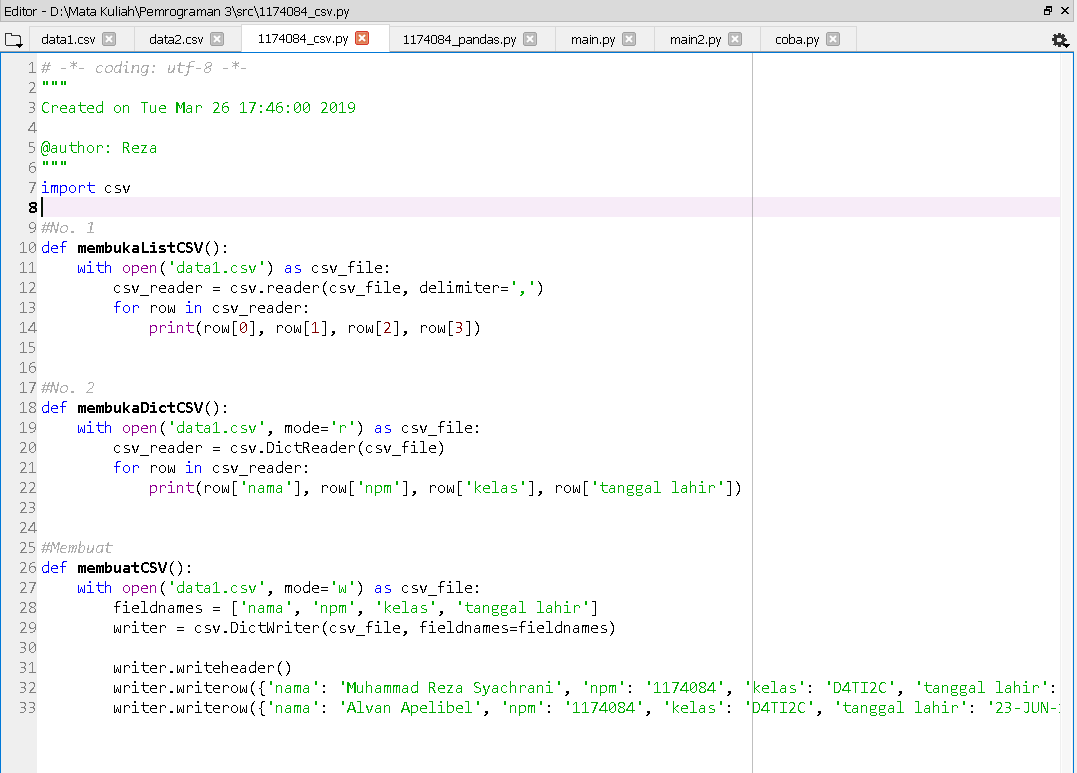
\includegraphics[width=5cm]{figures/4/1174084/Praktek/c4_1.png}
 \centering
\end{figure}

\begin{figure}[H]
 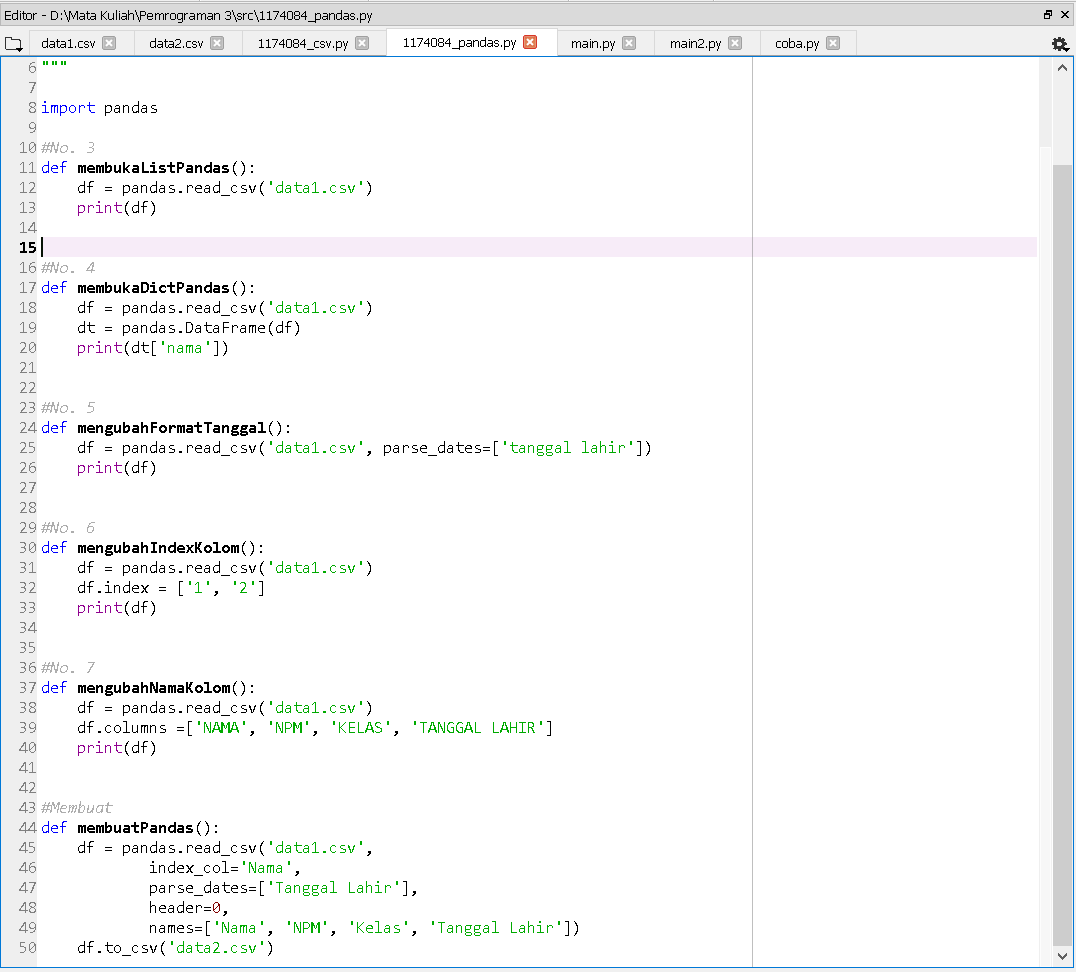
\includegraphics[width=5cm]{figures/4/1174084/Praktek/c4_2.png}
 \centering
\end{figure}

\begin{figure}[H]
 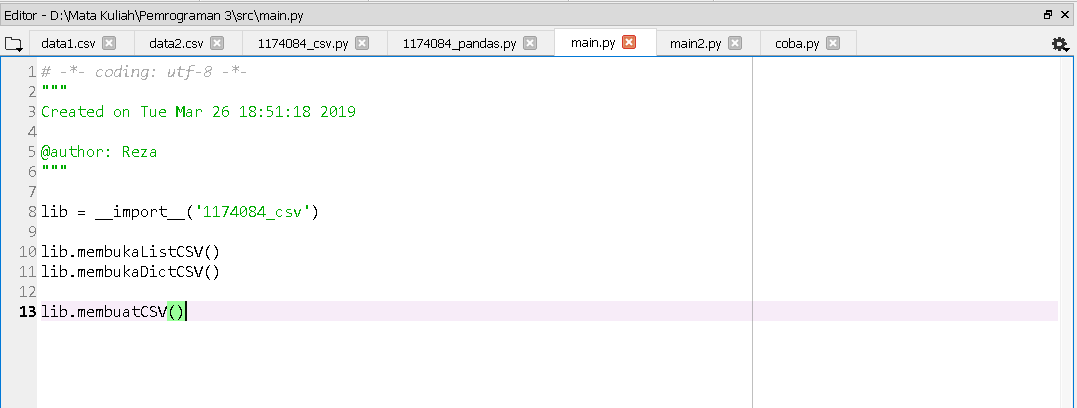
\includegraphics[width=5cm]{figures/4/1174084/Praktek/c4_3.png}
 \centering
\end{figure}

\begin{figure}[H]
 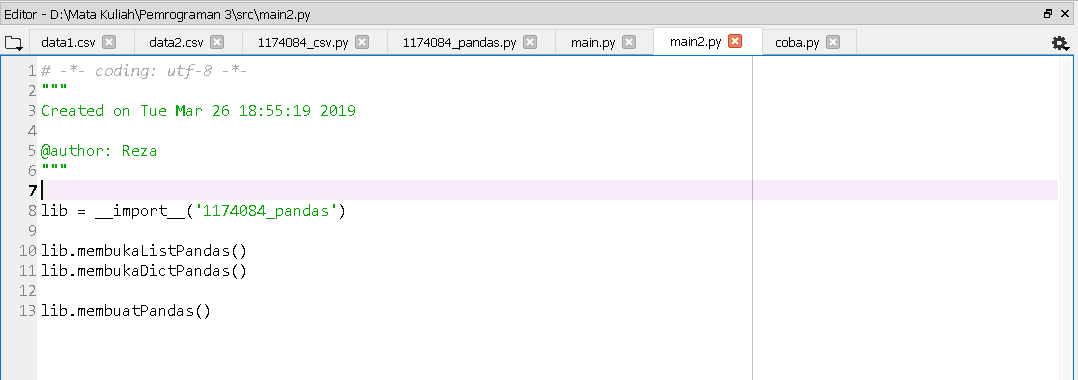
\includegraphics[width=5cm]{figures/4/1174084/Praktek/c4_4.png}
 \centering
\end{figure}

\begin{figure}[H]
 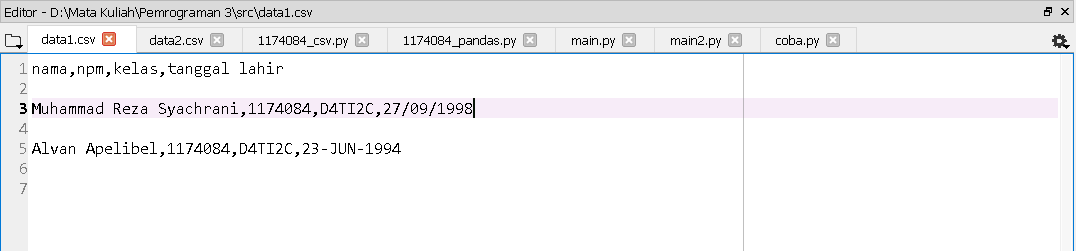
\includegraphics[width=5cm]{figures/4/1174084/Praktek/c4_5.png}
 \centering
\end{figure}

\begin{figure}[H]
 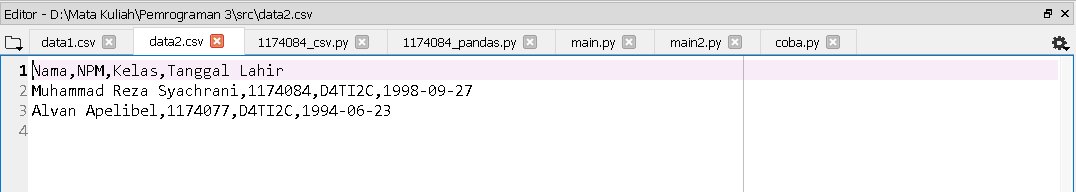
\includegraphics[width=5cm]{figures/4/1174084/Praktek/c4_6.png}
 \centering
\end{figure}

%%%%%%%%%%%%%%%%%%%%%%%%%%%%%%%%%%%%%%%%%%%%%%%%%%%%%%%%%%%%%%%%%%%%%%%%%%%%
\section{Advent Nopele Olansi Damiahan Sihite}
\subsection{Soal 1}
Buatlah  fungsi  (file  terpisah/library  dengan  nama  NPMcsv.py)  untuk  membuka file csv dengan lib csv mode list.

\lstinputlisting[caption = Fungsi untuk membuka file CSV dengan lib CSV mode list., firstline=10, lastline=15]{src/4/1174089/Praktek/1174089_csv.py}

\subsection{Soal 2}
Buatlah  fungsi  (file  terpisah/library  dengan  nama  NPMcsv.py)  untuk  membuka file csv dengan lib csv mode dictionary.

\lstinputlisting[caption =  Fungsi untuk membuka file CSV dengan lib CSV mode dictionary., firstline=17, lastline=22]{src/4/1174089/Praktek/1174089_csv.py}

\subsection{Soal 3}
Buatlah fungsi (file terpisah/library dengan nama NPMpandas.py) untuk membuka file csv dengan lib pandas mode list.

\lstinputlisting[caption =  Fungsi untuk membuka file CSV dengan lib Pandas mode list., firstline=10, lastline=13]{src/4/1174089/Praktek/1174089_pandas.py}

\subsection{Soal 4}
Buatlah fungsi (file terpisah/library dengan nama NPMpandas.py) untuk membuka file csv dengan lib pandas mode dictionary.

\lstinputlisting[caption =  Fungsi untuk membuka file CSV dengan lib Pandas mode dictionary., firstline=10, lastline=13]{src/4/1174089/Praktek/1174089_pandas.py}

\subsection{Soal 5}
Buat fungsi baru di NPMpandas.py untuk mengubah format tanggal menjadi standar dataframe.

\lstinputlisting[caption =  Fungsi untuk mengubah format tanggal menjadi standar dataframe., firstline=15, lastline=19]{src/4/1174089/Praktek/1174089_pandas.py}

\subsection{Soal 6}
Buat fungsi baru di NPMpandas.py untuk mengubah index kolom.

\lstinputlisting[caption =  Fungsi untuk mengubah index kolom., firstline=21, lastline=24]{src/4/1174089/Praktek/1174089_pandas.py}

\subsection{Soal 7}
Buat fungsi baru di NPMpandas.py untuk mengubah atribut atau nama kolom.

\lstinputlisting[caption =  Fungsi untuk mengubah atribut atau nama kolom., firstline=26, lastline=30]{src/4/1174089/Praktek/1174089_pandas.py}

\subsection{Soal 8}
Buat program main.py yang menggunakan library NPMcsv.py yang membuat dan membaca file csv.

\lstinputlisting[caption =  Membuat dan mebaca file CSV menggunakan library 1174006pandas., firstline=8, lastline=13]{src/4/1174089/Praktek/main.py}

\subsection{Soal 9}
Buat program main2.py yang menggunakan library NPMpandas.py yang membuat dan membaca file csv.

\lstinputlisting[caption = Membuat dan mmebaca file CSV menggunakan library 1174006pandas., firstline=8, lastline=13]{src/4/1174089/Praktek/main2.py}

\subsection{Kode Program Praktek}
\begin{figure}[H]
	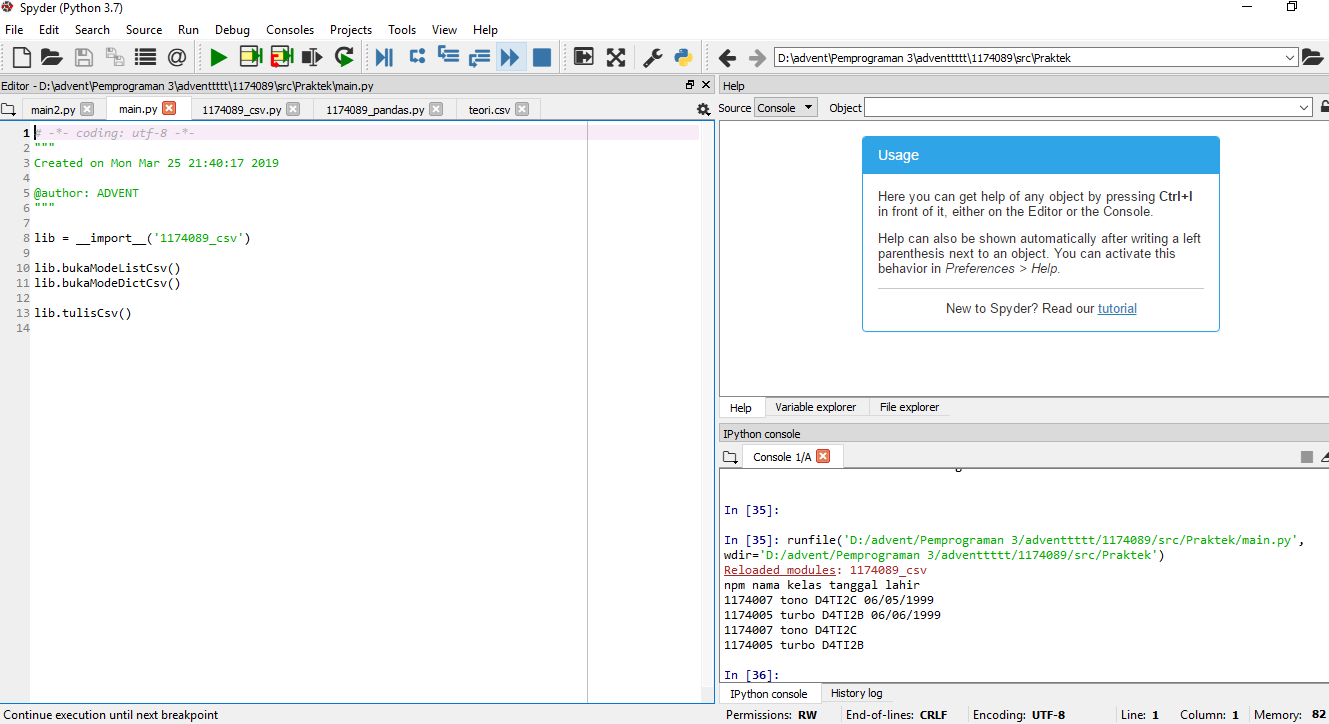
\includegraphics[width=9cm]{figures/4/1174089/Praktek/k1.png}
	\centering
\end{figure}
\begin{figure}[H]
	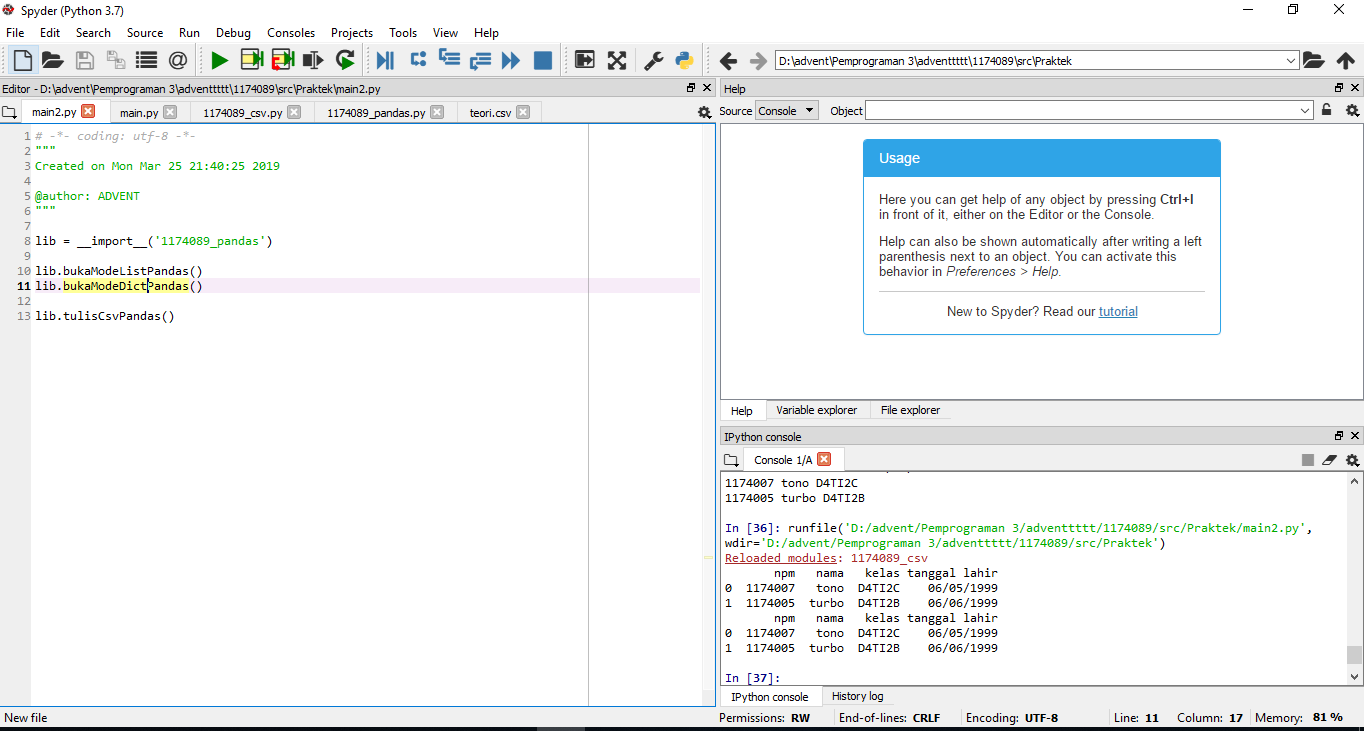
\includegraphics[width=10cm]{figures/4/1174089/Praktek/k2.png}
	\centering
\end{figure}
\begin{figure}[H]
	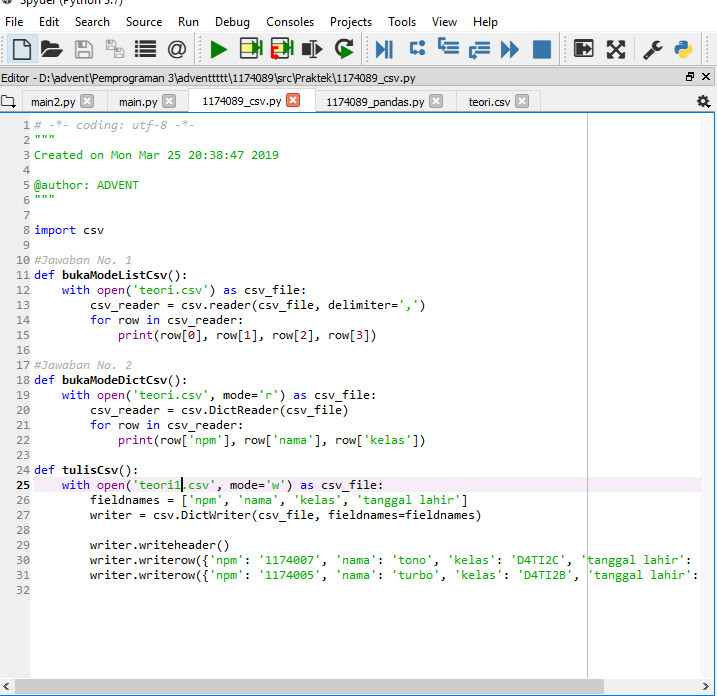
\includegraphics[width=10cm]{figures/4/1174089/Praktek/k3.png}
	\centering
\end{figure}
\begin{figure}[H]
	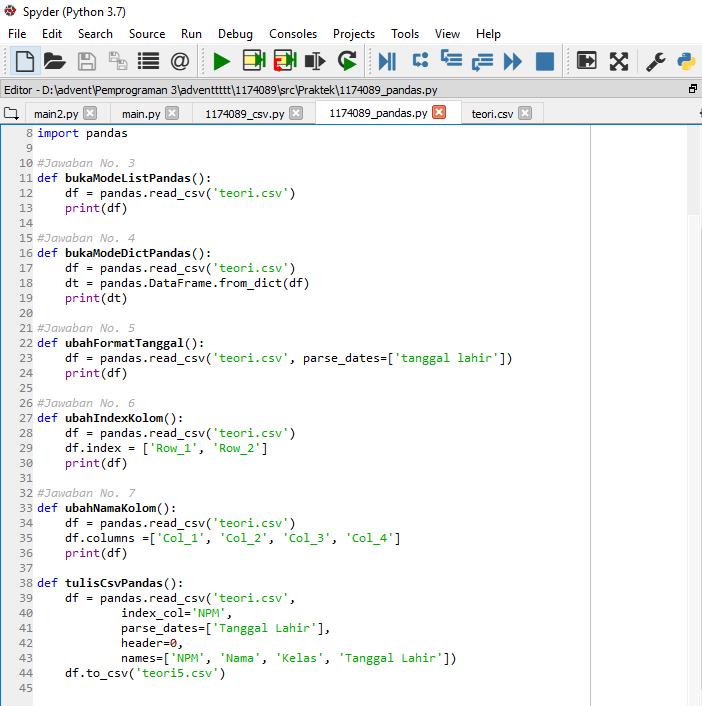
\includegraphics[width=9cm]{figures/4/1174089/Praktek/k4.png}
	\centering
\end{figure}
\begin{figure}[H]
	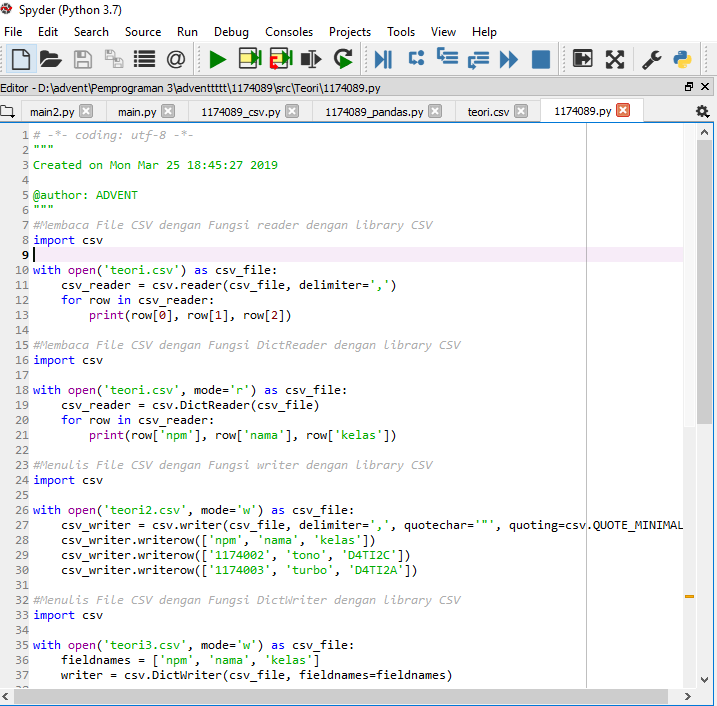
\includegraphics[width=10cm]{figures/4/1174089/Praktek/k5.png}
	\centering
\end{figure}

\subsection{Cek Plagiat Praktek}
\begin{figure}[H]
	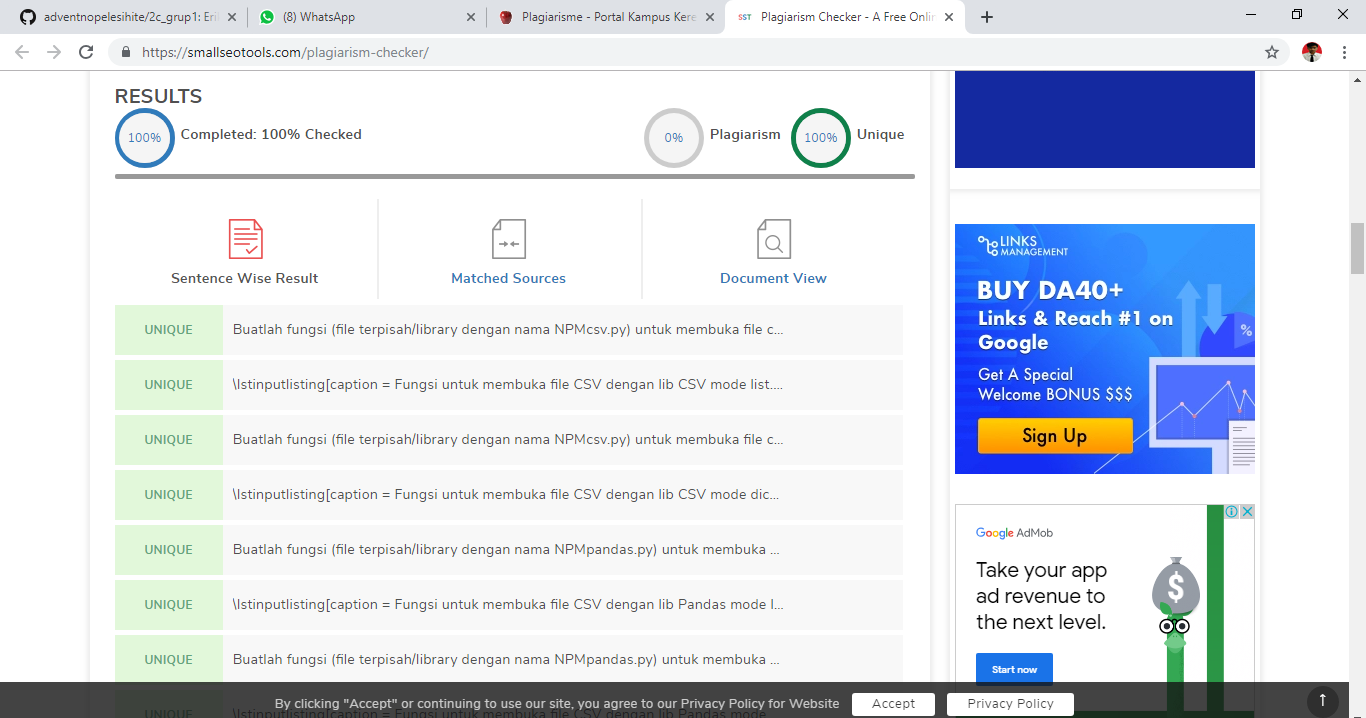
\includegraphics[width=10cm]{figures/4/1174089/Praktek/plagiatketerampilan.png}
	\centering
\end{figure}

\subsection{Soal 1}
Tuliskan  peringatan  error  yang  didapat  dari  mengerjakan  praktek  keempat  ini, dan  jelaskan  cara  penanganan  error  tersebut.   dan  Buatlah  satu  fungsi  yang menggunakan gunakan try except untuk menanggulangi error tersebut.

Peringatan error di praktek keempat ini, yaitu:
\begin{itemize}
	\item Syntax Errors
	Syntax Errors adalah suatu keadaan saat kode python mengalami kesalahan penulisan. Solusinya adalah memperbaiki penulisan kode yang salah.
	
	\item Name Error
	NameError adalah exception yang terjadi saat kode melakukan eksekusi terhadap local name atau global name yang tidak terdefinisi. Solusinya adalah memastikan variabel atau function yang dipanggil ada atau tidak salah ketik.
	
	\item Type Error
	TypeError adalah exception yang akan terjadi apabila pada saat dilakukannya eksekusi terhadap suatu operasi atau fungsi dengan type object yang tidak sesuai. Solusi dari error ini adalah mengkoversi varibelnya sesuai dengan tipe data yang akan digunakan.
\end{itemize}

Fungsi yang menggunakan try except
\lstinputlisting[caption= Fungsi yang menggunakan try except .,firstline=55, lastline=67]{src/4/1174089/Teori/1174089.py}

\subsection{Kode Program Penanganan Error}
\begin{figure}[H]
	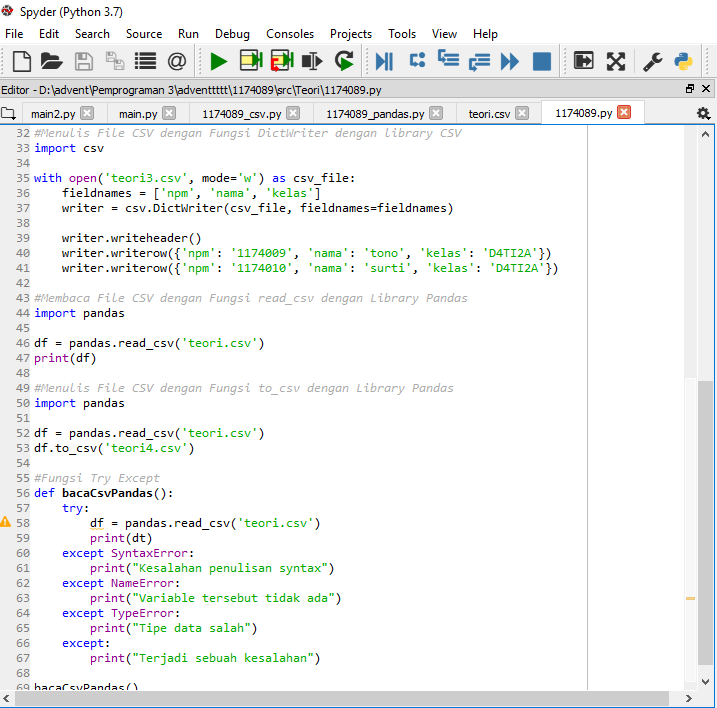
\includegraphics[width=10cm]{figures/4/1174089/Praktek/p1.png}
	\centering
\end{figure}

\subsection{Plagiat Penanganan Error}
\begin{figure}[H]
	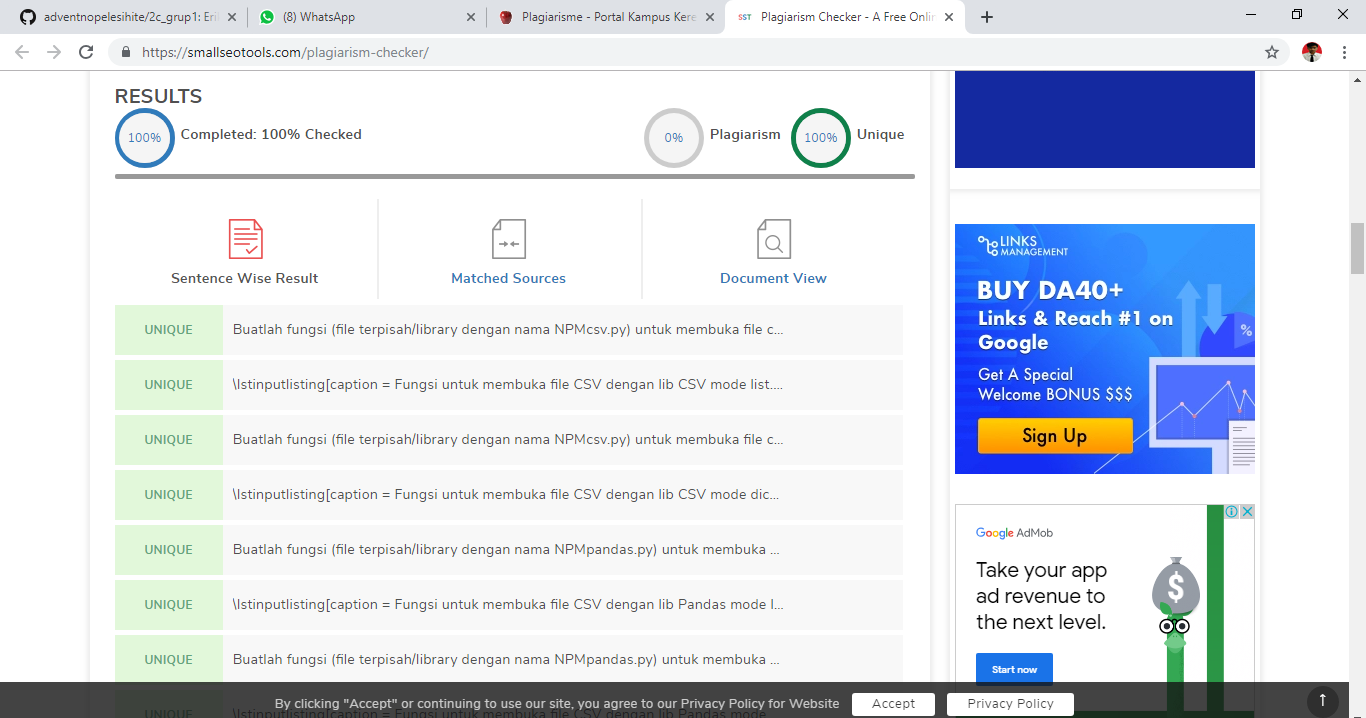
\includegraphics[width=10cm]{figures/4/1174089/Praktek/plagiatpenanganan.png}
	\centering
\end{figure}
%%%%%%%%%%%%%%%%%%%%%%%%%%%%%%%%%%%%%%%%%%%%%%%%%%%%%%%%%%%%%%%%%%%%%%%%%%%%%%%%%%%
\section{Arrizal Furqona Gifary}
\subsection{Praktek}
\begin{enumerate}

\item Buatlah fungsi (file terpisah/library dengan nama NPM csv.py) untuk membuka file csv dengan lib csv mode list
\lstinputlisting[firstline=10, lastline=20]{src/4/1174070/Praktek/d1174070_csv.py}

\item Buatlah fungsi (file terpisah/library dengan nama NPM csv.py) untuk membuka file csv dengan lib csv mode dictionary
\lstinputlisting[firstline=22,lastline=34]{src/4/1174070/Praktek/1174070_csv.py}

\item Buatlah fungsi (file terpisah/library dengan nama NPM pandas.py) untuk membuka file csv dengan lib pandas mode list
\lstinputlisting[firstline=7,lastline=10]{src/4/1174070/Praktek/d1174070_pandas.py}

\item Buatlah fungsi (file terpisah/library dengan nama NPM pandas.py) untuk membuka file csv dengan lib pandas mode dictionary
\lstinputlisting[firstline=12,lastline=15]{src/4/1174070/Praktek/d1174070_pandas.py}

\item Buat fungsi baru di NPM pandas.py untuk mengubah format tanggal menjadi standar dataframe
\lstinputlisting[firstline=17,lastline=19]{src/4/1174070/Praktek/d1174070_pandas.py}

\item Buat fungsi baru di NPM pandas.py untuk mengubah index kolom
\lstinputlisting[firstline=21,lastline=23]{src/4/1174070/Praktek/d1174070_pandas.py}

\item Buat fungsi baru di NPM pandas.py untuk mengubah atribut atau nama kolom
\lstinputlisting[firstline=25,lastline=29]{src/4/1174070/Praktek/d1174070_pandas.py}

\item Buat program main.py yang menggunakan library NPM csv.py yang membuat dan membaca file csv
\lstinputlisting[firstline=8,lastline=10]{src/4/1174070/Praktek/main_izal.py}

\item Buat program main2.py yang menggunakan library NPM pandas.py yang membuat dan membaca file csv
\lstinputlisting[firstline=12,lastline=14]{src/4/1174070/Praktek/main_izal.py}

\end{enumerate}
\begin{enumerate}
	\item Tuliskan  peringatan  error  yang  didapat  dari  mengerjakan  praktek  keempat  ini, dan  jelaskan  cara  penanganan  error  tersebut.   dan  Buatlah  satu  fungsi  yang menggunakan gunakan try except untuk menanggulangi error tersebut.
	
	Peringatan error di praktek keempat ini, yaitu:
	\begin{itemize}
		\item Syntax Errors
		Syntax Errors adalah suatu keadaan saat kode python mengalami kesalahan penulisan. Solusinya adalah memperbaiki penulisan kode yang salah.
		
		\item Name Error
		NameError adalah exception yang terjadi saat kode melakukan eksekusi terhadap local name atau global name yang tidak terdefinisi. Solusinya adalah memastikan variabel atau function yang dipanggil ada atau tidak salah ketik.
		
		\item Type Error
		TypeError adalah exception yang akan terjadi apabila pada saat dilakukannya eksekusi terhadap suatu operasi atau fungsi dengan type object yang tidak sesuai. Solusi dari error ini adalah mengkoversi varibelnya sesuai dengan tipe data yang akan digunakan.
	\end{itemize}

\end{enumerate}

%%%%%%%%%%%%%%%%%%%%%%%%%%%%%%%%%%%%%%%%%%%%%%%%%%%%%%%%%%%%%%%%%%%%%%%%%%%%%%%%%%%%%%%%%%%%%%%%%%%%
\section{Mochamad Arifqi Ramadhan | 1174074}
\subsection{Pengelolaan File CSV (Keterampilan Pemrograman)}
\begin{enumerate}
    \item Buatlah  fungsi  (file  terpisah/library  dengan  nama  \verb|NPM_csv.py|)  untuk  membuka file csv dengan lib csv mode list.
    
    \lstinputlisting[firstline=8, lastline=14]{src/4/1174074/Praktek/1174074_csv.py}

    \item Buatlah  fungsi  (file  terpisah/library  dengan  nama  \verb|NPM_csv.py|)  untuk  membuka file csv dengan lib csv mode dictionary.
   	
   	\lstinputlisting[firstline=16, lastline=20]{src/4/1174074/Praktek/1174074_csv.py}

	\item Buatlah fungsi (file terpisah/library dengan nama \verb|NPM_pandas.py|) untuk membuka file csv dengan lib pandas mode list.
	
	\lstinputlisting[firstline=7, lastline=11]{src/4/1174074/Praktek/1174074_pandas.py}
		
	\item Buatlah fungsi (file terpisah/library dengan nama \verb|NPM_pandas.py| untuk membuka file csv dengan lib pandas mode dictionary.

	\lstinputlisting[firstline=13, lastline=16]{src/4/1174074/Praktek/1174074_pandas.py}

	\item Buat fungsi baru di \verb|NPM_pandas.py| untuk mengubah format tanggal menjadi standar dataframe.

	\lstinputlisting[firstline=25, lastline=27]{src/4/1174074/Praktek/1174074_pandas.py}

	\item Buat fungsi baru di \verb|NPM_pandas.py| untuk mengubah index kolom.
	
	\lstinputlisting[firstline=29, lastline=32]{src/4/1174074/Praktek/1174074_pandas.py}
	
	\item Buat fungsi baru di \verb|NPM_pandas.py| untuk mengubah atribut atau nama kolom.
	
	\lstinputlisting[firstline=34, lastline=37]{src/4/1174074/Praktek/1174074_pandas.py}
	
	\item Buat program main.py yang menggunakan library \verb|NPM_csv.py| yang membuat dan membaca file csv.
	
	\lstinputlisting[firstline=8, lastline=15]{src/4/1174074/Praktek/main.py}
	
	\item Buat program main2.py yang menggunakan library \verb|NPM_pandas.py| yang membuat dan membaca file csv.

	\lstinputlisting[firstline=8, lastline=12]{src/4/1174074/Praktek/main2.py}
\end{enumerate} 

\subsection{Keterampilan Penanganan Error}

\begin{enumerate}
	\item Tuliskan peringatan error yang didapat dari mengerjakan praktek ketiga ini,
dan jelaskan cara penanganan error tersebut. dan Buatlah satu fungsi yang
menggunakan gunakan try except untuk menanggulangi error tersebut.

	\lstinputlisting[firstline=7, lastline=16]{src/4/1174074/Praktek/error.py}
	
	\par NameError adalah exception yang terjadi saat kode melakukan eksekusi terhadap local name atau global name yang tidak terdefinisi. Misalnya saat menjumlahkan variable yang tidak didefinisikan, memanggil function yang tidak ada, dan lain-lain.
	
\end{enumerate}

\textbf{Screenshoot Kode Program Python}

\begin{figure}[H]
 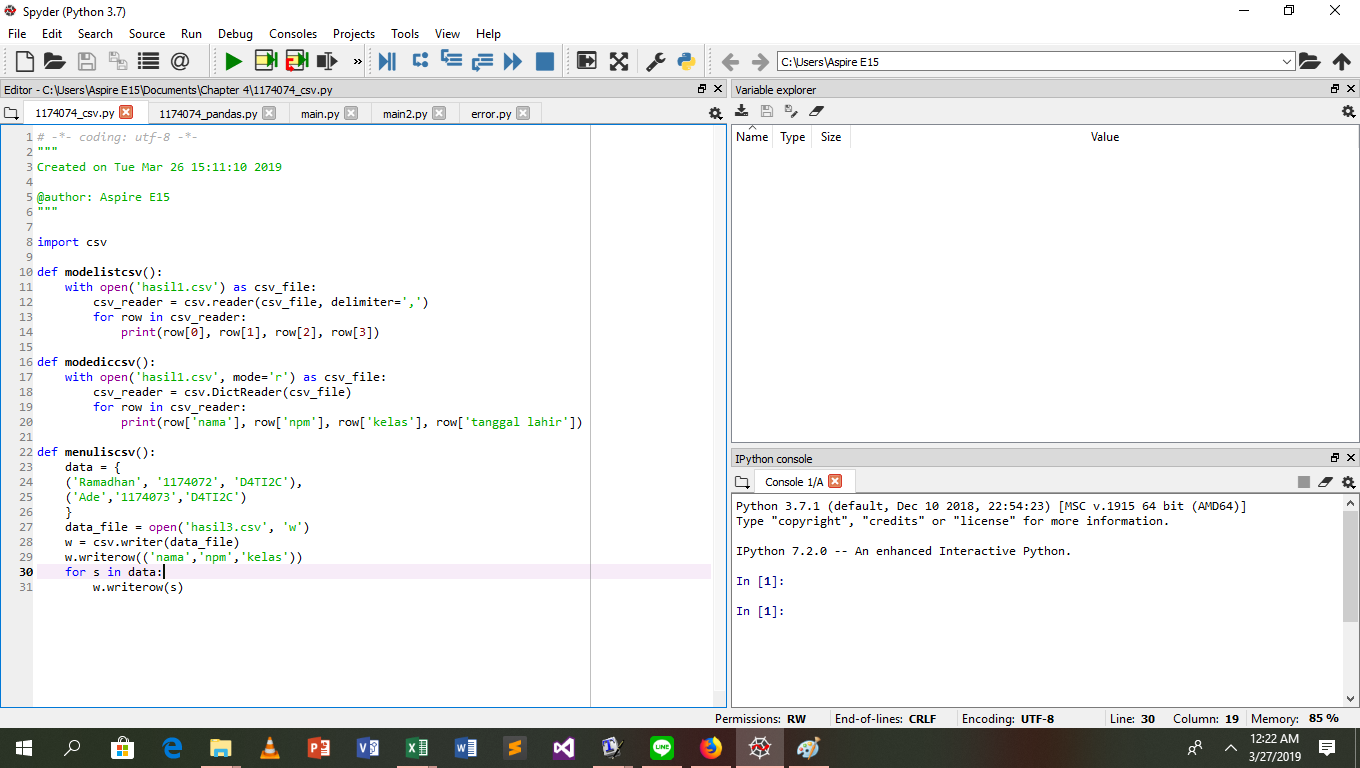
\includegraphics[width=5cm]{figures/4/1174074/Praktek/csv.png}
 \centering
\end{figure}

\begin{figure}[H]
 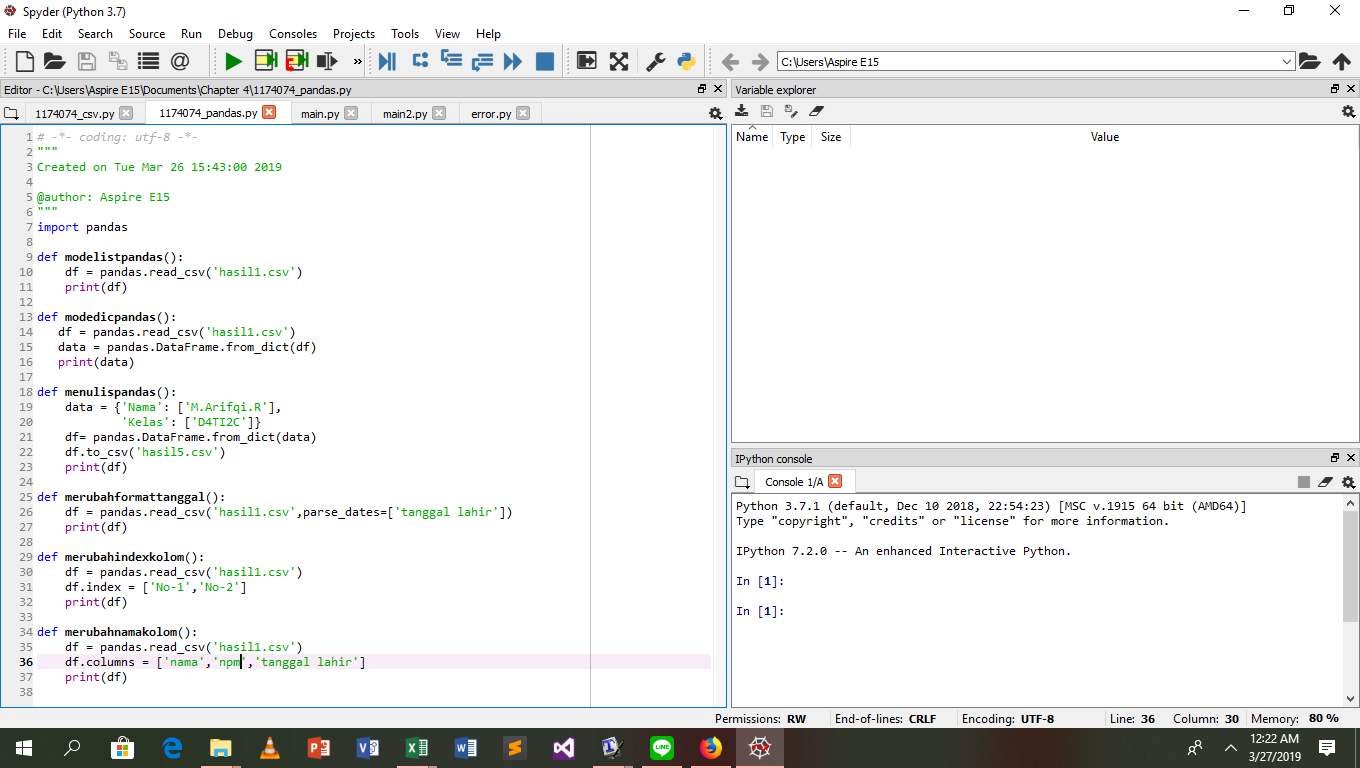
\includegraphics[width=5cm]{figures/4/1174074/Praktek/pandas.png}
 \centering
\end{figure}

\begin{figure}[H]
 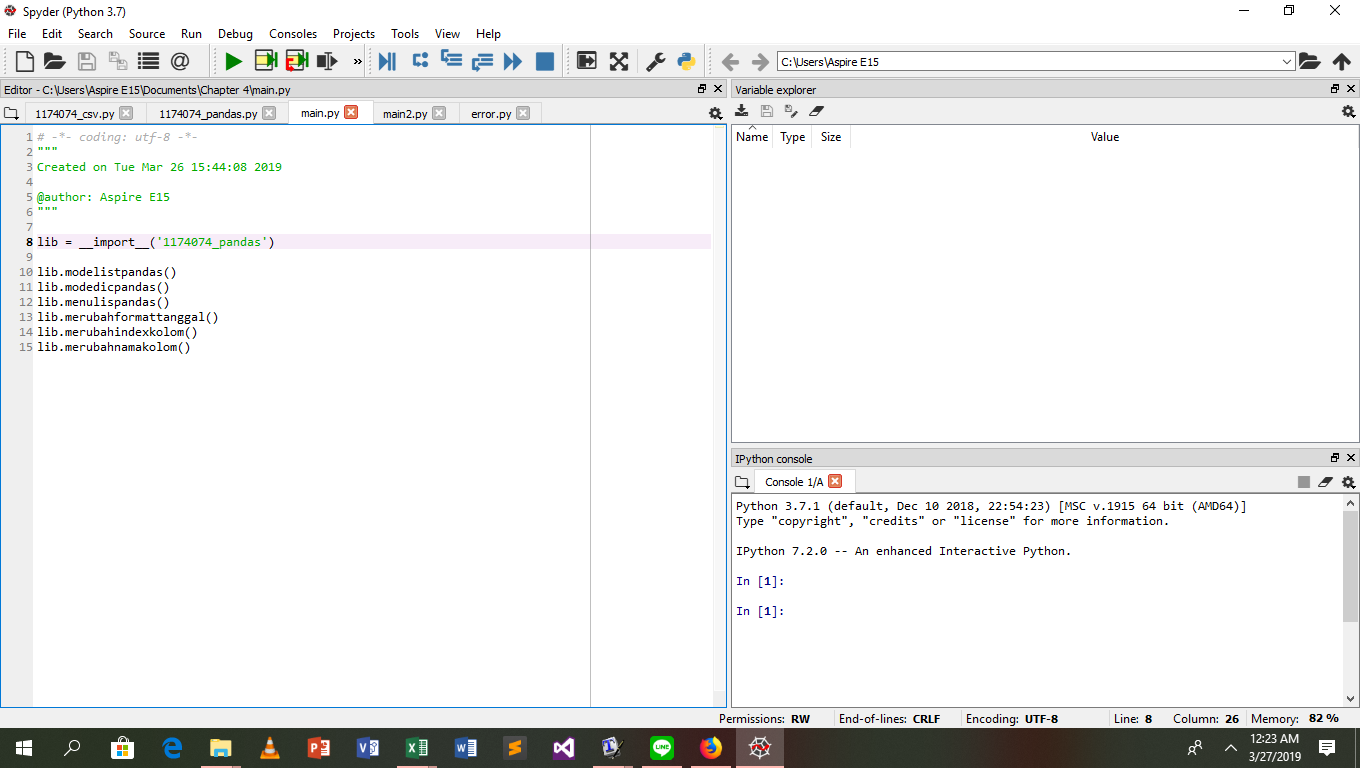
\includegraphics[width=5cm]{figures/4/1174074/Praktek/main.png}
 \centering
\end{figure}

\begin{figure}[H]
 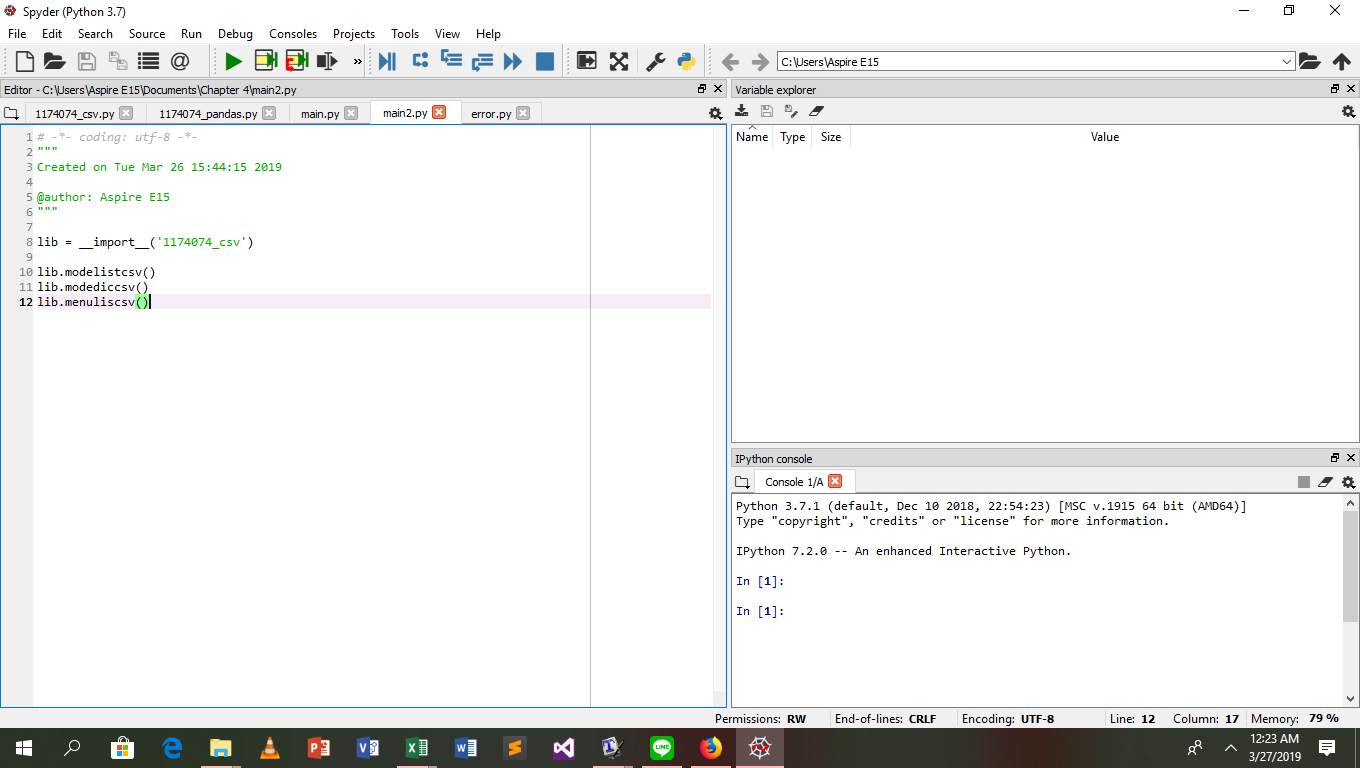
\includegraphics[width=5cm]{figures/4/1174074/Praktek/main2.png}
 \centering
\end{figure}

\begin{figure}[H]
 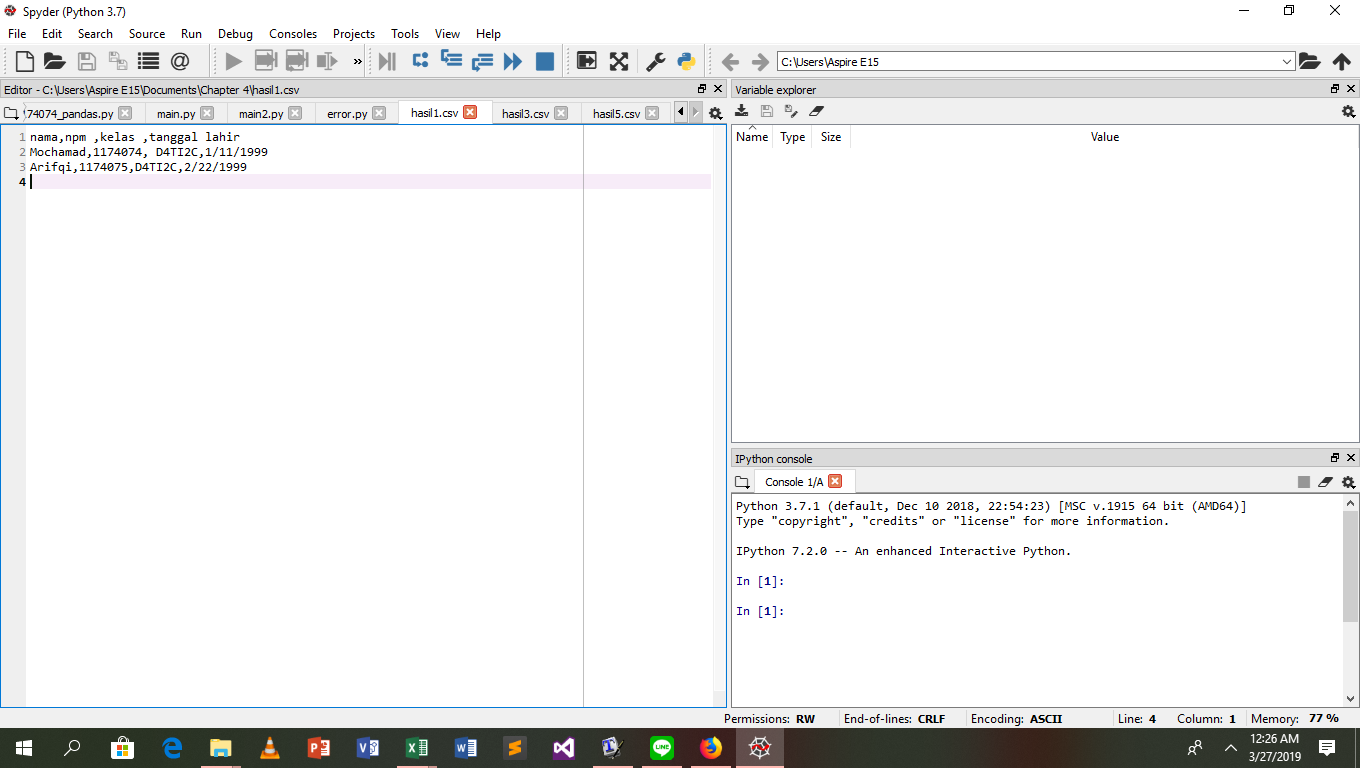
\includegraphics[width=5cm]{figures/4/1174074/Praktek/hasil1.png}
 \centering
\end{figure}

\begin{figure}[H]
 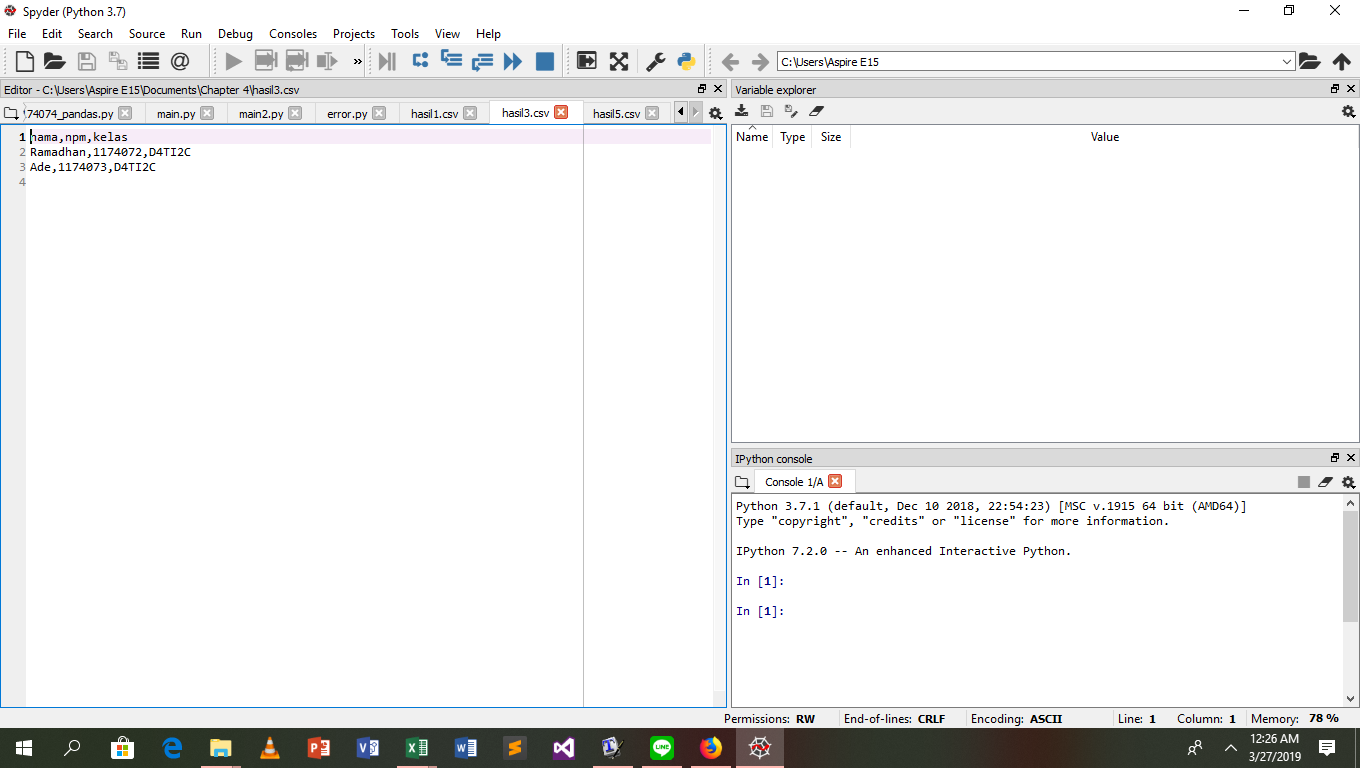
\includegraphics[width=5cm]{figures/4/1174074/Praktek/hasil3.png}
 \centering
\end{figure}

\begin{figure}[H]
 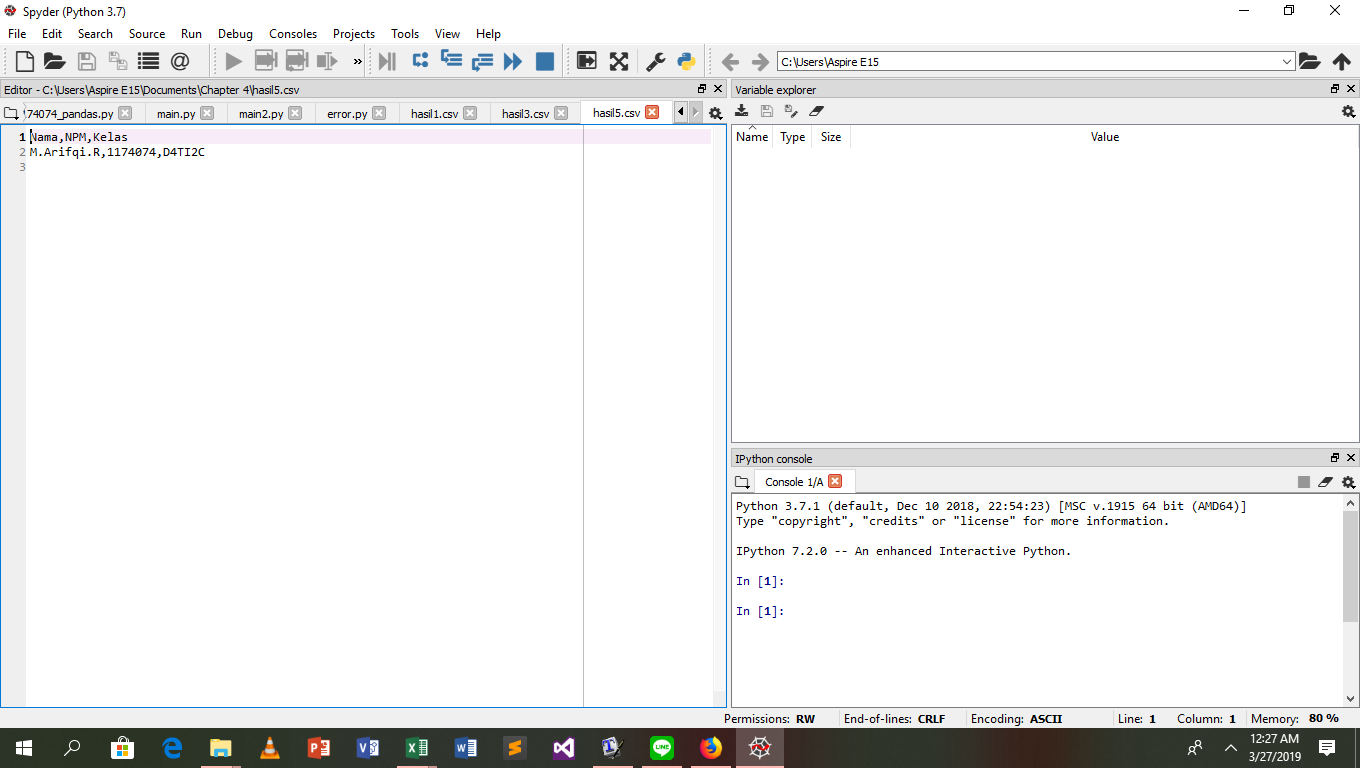
\includegraphics[width=5cm]{figures/4/1174074/Praktek/hasil5.png}
 \centering
\end{figure}

\begin{figure}[H]
 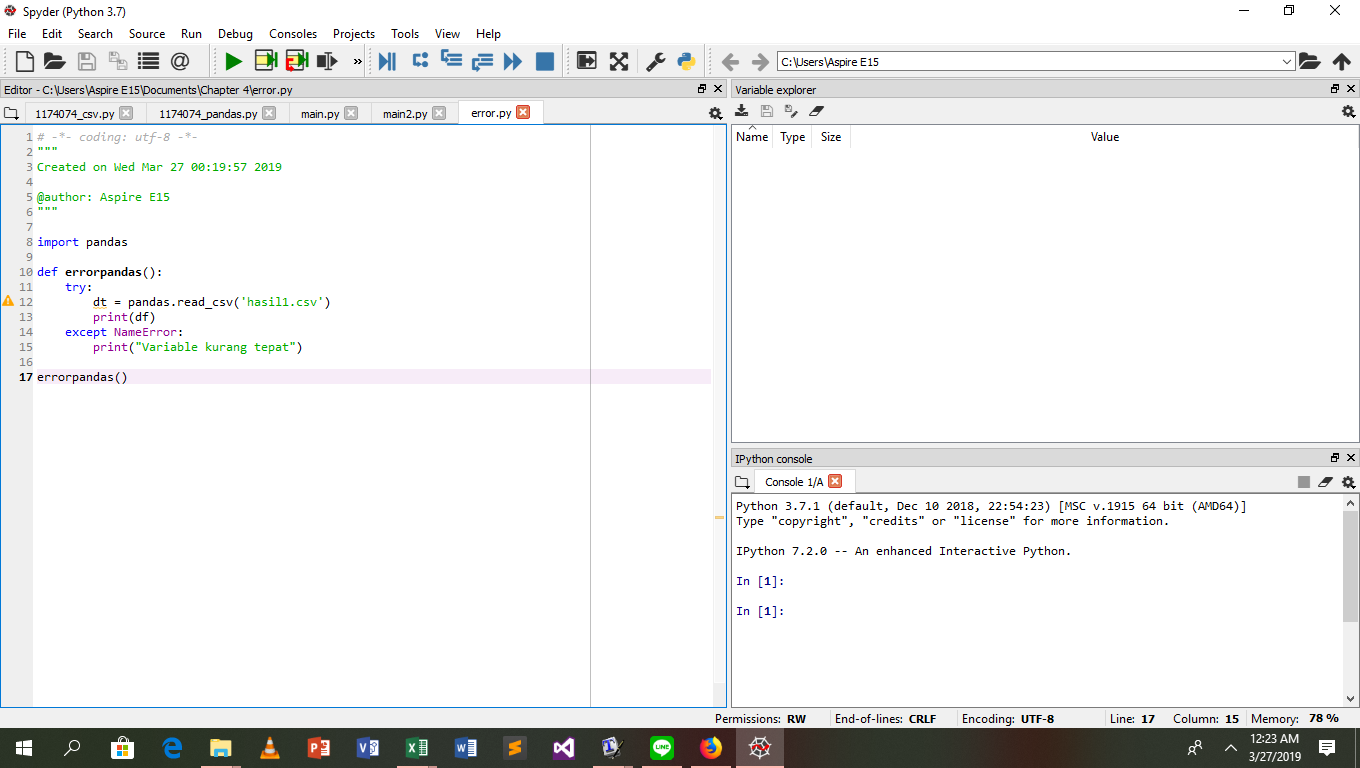
\includegraphics[width=5cm]{figures/4/1174074/Praktek/error.png}
 \centering
\end{figure}
%%%%%%%%%%%%%%%%%%%%%%%%%%%%%%%%%%%%%%%%%%%%%%%%%%%%%%%%%%%%%%%%%%%%%%%%%%%%%%%%%%%%%%%%%%%%%%%%%%%%%%%%%%%%%%%%%
\section{Engelbertus Adiputra Mau Leto}
 \subsection{Keterampilan Pemograman}
\begin{enumerate}
    \item Buatlah fungsi (file terpisah/library dengan nama NPM csv.py) untuk mem-
    buka file csv dengan lib csv mode list
    Berikut adalah pemanggilan file csv dengan library csv yang menggunakan list
    \lstinputlisting[firstline=10, lastline=20]{src/4/1174078/Praktek/c_1174078_csv.py}
    \item Buatlah fungsi (file terpisah/library dengan nama NPM csv.py) untuk mem-
    buka file csv dengan lib csv mode dictionary
    Berikut adalah pemanggilan file csv dengan library csv yang menggunakan dictionary
    \lstinputlisting[firstline=22, lastline=31]{src/4/1174078/Praktek/c_1174078_csv.py}
    \item Buatlah fungsi (file terpisah/library dengan nama NPM pandas.py) untuk mem-
    buka file csv dengan lib csv mode list
    Berikut adalah pemanggilan file csv dengan library pandas yang menggunakan list
    \lstinputlisting[firstline=9, lastline=11]{src/4/1174078/Praktek/p_1174078_pandas.py}
    \item Buatlah fungsi (file terpisah/library dengan nama NPM pandas.py) untuk mem-
    buka file csv dengan lib csv mode dictionary
    Berikut adalah pemanggilan file csv dengan library pandas yang menggunakan dictionary
    \lstinputlisting[firstline=13, lastline=16]{src/4/1174078/Praktek/p_1174078_pandas.py}
    \item Buat fungsi baru di NPM pandas.py untuk mengubah format tanggal menjadi
    standar datar frame
    Berikut penggunaan untuk merubah standar penulisan tanggal, yang mengikuti standar penulisan dari pandas.
    \lstinputlisting[firstline=18, lastline=20]{src/4/1174078/Praktek/p_1174078_pandas.py}
    \item Buat fungsi baru di NPM pandas.py untuk mengubah index kolom
    Berikut merupakan pergantian index kolom
    \lstinputlisting[firstline=22, lastline=24]{src/4/1174078/Praktek/p_1174078_pandas.py}
    \item Buat fungsi baru di NPM pandas.py untuk mengubah atribut atau nama kolom
    berikut merupakan penggunaan untuk merename atribut yang digunakan, atau merubah nama header 0
    \lstinputlisting[firstline=26, lastline=30]{src/4/1174078/Praktek/p_1174078_pandas.py}
    \item Buat program main.py yang menggunakan library NPM csv.py yang membuat
    dan membaca file csv
    \lstinputlisting[firstline=8, lastline=10]{src/4/1174078/Praktek/main_engel.py}
    \item Buat program main2.py yang menggunakan library NPM pandas.py yang mem-
    buat dan membaca file csv
    \lstinputlisting[firstline=11, lastline=14]{src/4/1174078/Praktek/main_engel.py}

\subsection{Kode Program Praktek}
\begin{figure}[H]
	\includegrapichs[width=10cm]{figures/4/1174078/Prakter/c1.png}
	\centering
\end{figure}
\begin{figure}[H]
	\includegrapichs[width=10cm]{figures/4/1174078/Prakter/c2.png}
	\centering
\end{figure}
\begin{figure}[H]
	\includegrapichs[width=10cm]{figures/4/1174078/Prakter/c3.png}
	\centering
\end{figure}
\begin{figure}[H]
	\includegrapichs[width=10cm]{figures/4/1174078/Prakter/c4.png}
	\centering
\end{figure}
\begin{figure}[H]
	\includegrapichs[width=10cm]{figures/4/1174078/Prakter/c5.png}
	\centering
\end{figure}
\begin{figure}[H]
	\includegrapichs[width=10cm]{figures/4/1174078/Prakter/c6.png}
	\centering
\end{figure}

\subsection{Cek Plagiat Praktek}
\begin{figure}[H]
	\includegrapichs[width=10cm]{figures/4/1174078/Prakter/c7.png}
	\centering
\end{figure}
\subsection{Penangganan error}
dalam praktek kali ini Puji Tuhan tidak menemukan error
\end{enumerate}

%%%%%%%%%%%%%%%%%%%%%%%%%%%%%%%%%%%%%%%%%%%%%%%%%%%%%%%%%%%%%%%%%%%